%
% File: EFT.tex
% Author: Ran Itay
% Description: EFT analysis
%
\let\textcircled=\pgftextcircled
\chapter{Effective Field Theory Search for High Energy Nuclear Recoils in \textsc{Xenon100} Detector}
\label{chap:EFT}

\initial{S}tandard SI,SD analysis concentrate on energy recoils of up to O(10)\,$\keVr$, hence a hard high energy threshold is used for them. In \textsc{Xenon100} this threshold value is 43\,$\keVr$. However SI and SD are not the only types of interactions possible. These new interactions which predicts higher recoil energies are considered in the EFT framework (see ~\ref{sec:intro_EFT}). Moreover a WIMP may have several mass states, which may also result in a possible higher energy recoil. In Fig.~\ref{fig:EFTdrde} is an example of an expected recoil spectrum from different operators. 

\begin{figure}[t!]
	\centering
	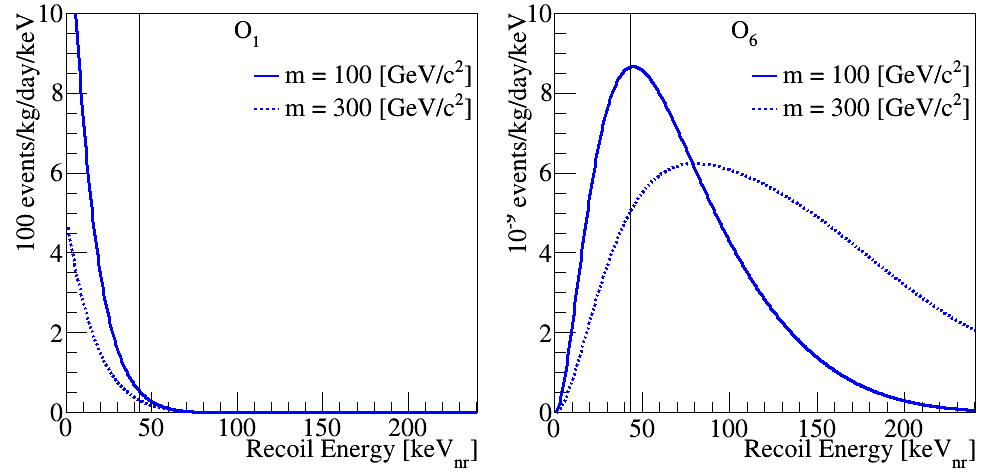
\includegraphics[width=0.8\textwidth]{fig/drde.png}
	\mycaption[drde for example operators.]{Example EFT recoil spectra for elastic scattering of spin-$1/2$ WIMPs on Xenon nuclei (weighted according to the isotope abundances in the \textsc{Xenon100} experiment). Left(right) shows the predicted spectra for EFT operator $\mathcal{O}_1$($\mathcal{O}_6$). The normalization is controlled by the coupling coefficient of each EFT operator and the experimental exposure. The solid vertical line at $43~\keVr$ shows the approximate division between the two signal regions used in this analysis. As shown, the standard SI ($\mathcal{O}_1$) spectrum is concentrated mainly in the already explored energy region. However, some EFT operators, for certain WIMP masses, predict a significant fraction of recoil events above the upper energy cut used in the standard SI analysis, motivating an extension of this cut. The highest recoil energy shown in the plots, $240~\keVr$, roughly corresponds to the highest energy accounted for this analysis.}
	\label{fig:EFTdrde}
\end{figure}

	    
The EFT framework of \cite{Fitzpatrick:2012ib} is constructed at the WIMP-nucleon level and so each operator may be present independently for protons and neutrons, though UV models can of course correlate their couplings. The full EFT thus has 28 coupling parameters in addition to the WIMP mass, plus a mass splitting~$\delta$ in the inelastic case. This parameter space is too large to explore in full, so a similar approach to the SI/SD case is taken, assuming only one active operator at a time, considering it equally coupled to protons and neutrons (the ``isoscalar'' case). 

To facilitate the full exploitation of these results by the community, I provide in supplementary material a set of tools for converting any theoretical recoil spectrum $\mathrm{d}R/\mathrm{d}E$ into an accurate event rate prediction for this analysis, including all detector response and analysis efficiency effects. This may help to set a mildly conservative but quite accurate limit on arbitrary models in the full EFT parameter space, or any other particle dark matter model for which one can supply the expected recoil spectrum. These tools are described further in Appendix~\ref{app:response_table}.
%=======

In this work I reanalyze science run~II data recorded between February 2011 and March 2012, corresponding to 224.6~live~days. The characterization of the detector response to ER interactions is performed using dedicated calibration campaigns with $^{60}$Co and $^{232}$Th radioactive sources, while the response to NR interactions is performed using $^{241}$AmBe neutron source calibration campaigns.
 
This work extends the previous results~\cite{xe100_run10_si,xe100_run_combination}, referred to in the following as the low-energy channel, with a new study exploring the recoil energy range between $(43-240)~\keVr$. 
The data analysis is divided into two mutually exclusive channels, one optimized for low energies and ranging from $(3-30)$~PE in \cSi{} (low-energy), 
and the other optimized for high energies recoils ranging from $(30-180)$~PE in \cSi{} (high-energy). These two analyses are then combined statistically. 


\section{Low Energy Channel}
\label{subsec:LowE}
This analysis channel relies on the reanalysis of run~II data described in~\cite{xe100_run_combination}. The Region Of Interest (ROI), background 
expectation models, data selections and their acceptances are mostly unchanged and so are only briefly summarized here. Differences with respect to said results are highlighted when present.

The ROI for this channel is defined in the (log$(\cSiib{}/\cSi{}),\cSi{}$)-plane and is shown in Fig.~\ref{fig:phasespace}.  The lower 
bound on log$(\cSiib{}/\cSi{})$ corresponds to a 3\,$\sigma$ acceptance quantile (as a function of \cSi{}) of a 20~GeV WIMP mass signal model assuming an $\mathcal{O}_1$ (SI) interaction, while the upper bound is fixed at log$(\cSiib{}/\cSi{})=2.7$.
The range in \cSi{} is selected as ($3-30$)\,PE. 
The ROI is further divided into eight subregions (also called bands) depending on the operator $\mathcal{O}_i$ and on the WIMP mass hypothesis. 
These bands are arranged to achieve constant expected signal density in each region, as described in~\cite{xe100_run_combination}.

\begin{figure}[]
\begin{minipage}{1\linewidth}
\centerline{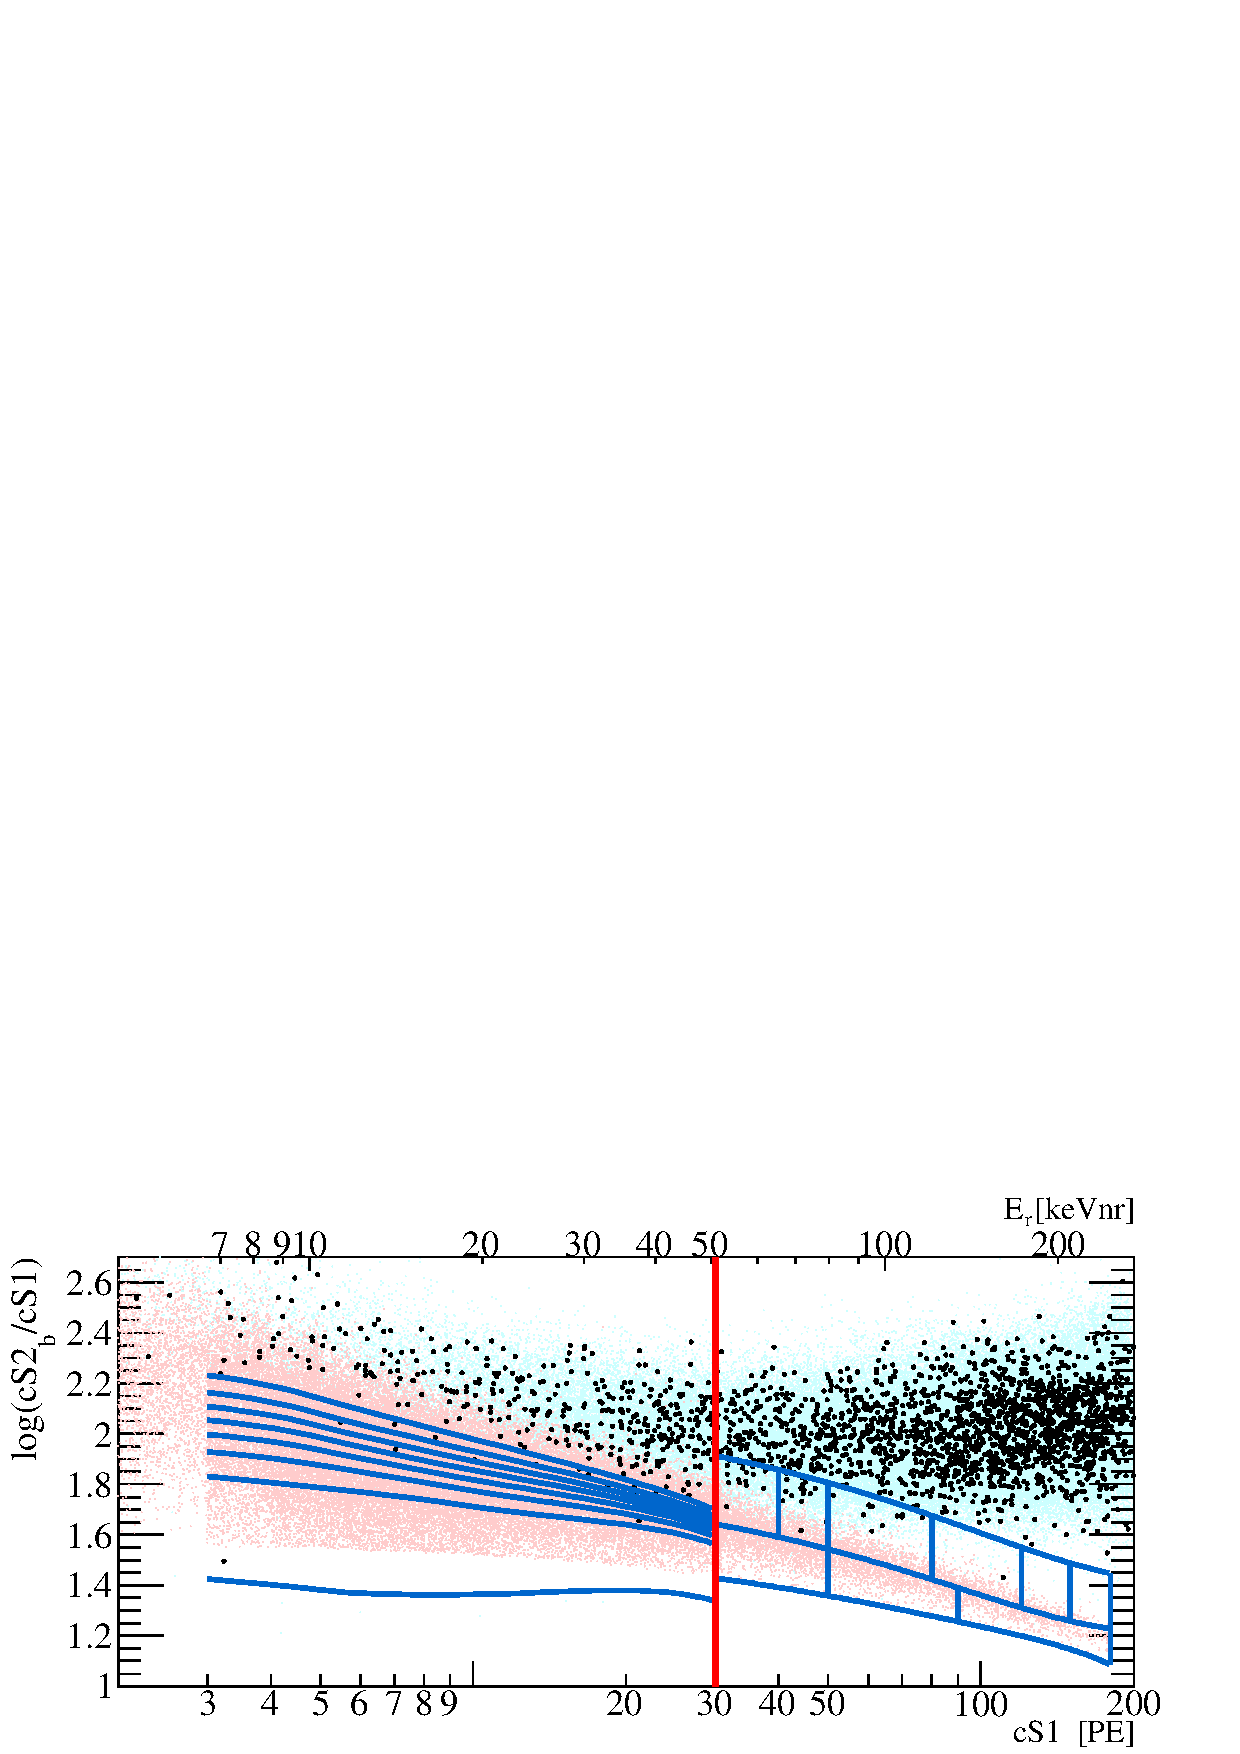
\includegraphics[width=1\linewidth]{fig/eft_sr.pdf}}
\end{minipage}
\mycaption[Summary of regions of interest backgrounds, and observed data]{Summary of regions of interest, backgrounds, and observed data. ER calibration data, namely $^{60}\mathrm{Co}$ and $^{232}\mathrm{Th}$ data are shown as light cyan dots. NR calibration data ($^{241}$AmBe) are shown as light red dots. Dark matter search data is shown as black dots. The red line is the threshold between the low- and high-energy channels. The lines in blue are the bands. For the low-energy channel, the bands are constructed to achieve constant expected signal density, and are operator and mass dependent, shown here for a 50~GeV/$c^2$ WIMP using the $\mathcal{O}_1$ operator. For the high-energy region, the nine analysis bins are presented also in blue lines.
}
\label{fig:phasespace}
\end{figure}  


Other than falling into the ROI, an event should fulfill several additional selection criteria (cuts). Data quality and selection cuts are defined to remove events with poor data quality or noisy signals. Events are discarded if they present a time-coincident signal in the outer LXe veto, \Sii{} signals below threshold, multiple-scatters, or are localized outside a predefined fiducial volume of 34 kg. In addition, this analysis channel uses the postunblinding cuts and data reprocessing described in~\cite{xe100_run_combination}. More details on these selection criteria and their relative WIMP signals acceptances can be found in~\cite{Aprile:2012vw,xe100_run_combination}. 

%%%%%%%%%%%%%%%%%%%%%%%%%%%%%%%%%%%%%%%%%%%%%
Note that this analysis channel does not employ a variable lower \Si{} threshold as a function of the event position in the TPC but instead applies a fixed lower threshold cut on \cSi{} at 3\,PE, conversely to the choice made in~\cite{xe100_run_combination}.

The expected background is modeled separately for ER and NR contributions which are then scaled to exposure and added together.
The NR background is estimated by Monte Carlo simulation and accounts for the radiogenic and cosmogenic neutron
contributions~\cite{Aprile:2013tov}. The ER background is parametrized as the linear combination of Gaussian-shaped and non-Gaussian components.
The former is obtained via a parametric fit of the $^{60}$Co and $^{232}$Th calibration data, as discussed in~\cite{xe100_run10_si}.

The latter, which consist of anomalous events such as those 
presenting incomplete charge collection or accidental coincidence of uncorrelated \Si{}s and \Sii{}s,  
is evaluated via dedicated techniques described in~\cite{xe100_run_combination}.

Systematic uncertainties on the background model arising from the Gaussian parametrized fit, and from the normalizations of the NR and non-Gaussian components, have been evaluated and propagated to each band. 
These errors are small with respect to the statistical uncertainties of each band, which are conservatively taken as the overall uncertainty~\cite{xe100_run_combination}, as discussed in Sec.~\ref{sec:LikelihoodFunction}.



\section{High Energy Channel}
\label{subsubsec:HighE}
This analysis channel targets high-energy nuclear recoils and is the focus of this work. The data selection criteria used are based on the criteria described in detail in \cite{Aprile:2012vw}, which were optimized for high acceptance to low-energy nuclear recoils. Most of these cuts were found to be fully compatible with (or easily extended) to high energy depositions; however some required more comprehensive studies, which are described in the following . 

The width of an \Sii{} pulse increases with the depth (z) of the interaction. This is due to the diffusion of the electron cloud during its propagation
through the liquid xenon. Since low-energy \Sii{} events show larger spread
due to low statistics of drifted electrons, the cut was previously defined in an energy-dependent way. However, for the large recoil energies considered in this channel, this energy dependency is no longer valid. I therefore use here a cut on the \Sii{} width which is a function of the depth of the interaction alone. 

As a WIMP will interact only once in the detector, I remove events which have more than one \Sii{}. I adopt in this analysis a cut that is more suitable to higher energies and demand a single \Sii{} in a 160 $\mu$s window, instead of a linear dependence between the second \Sii{} size and the first. 

To define the interaction's exact location in ($x,y$), I use several algorithms, one of which is based on a neural network (NN)~\cite{Aprile:2012vw}. The NN was not trained to recognize high energy ER events, and therefore a cut on the NN reconstruction quality is not suitable for this analysis. I therefore discard this cut but keep all other selections on position reconstruction quality, which is sufficient to ensure a correct position reconstruction. 

The total acceptance to WIMP signals is computed based on $^{241}$AmBe calibration data as a function of \cSi, following the procedure described in~\cite{Aprile:2012vw}. I present this function in Fig.~\ref{fig:Acc}, where the total acceptance is fitted using a third-order polynomial.

\begin{figure}[t!]
\begin{minipage}{0.9\linewidth}
\centerline{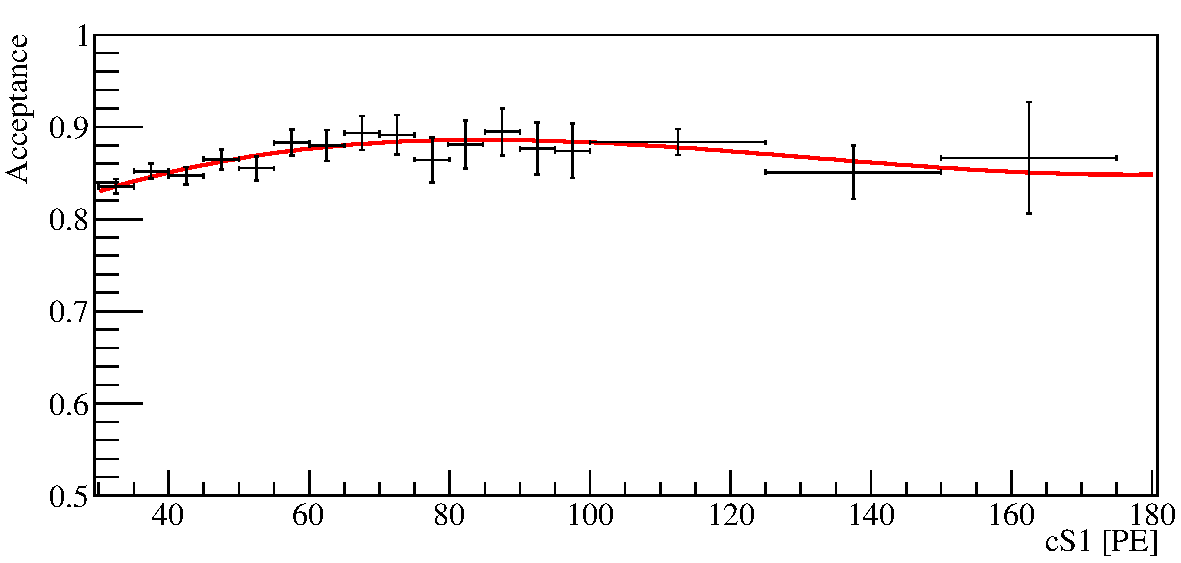
\includegraphics[width=1.\linewidth]{fig/Acceptance.pdf}}
\end{minipage}
\mycaption[The total acceptance of all cuts used]{The total acceptance of all cuts used. Data from calibration are shown in black, with a third-order polynomial fit in red.}
\label{fig:Acc}
\end{figure}

I define our signal region in the discrimination log$(\cSiib{}/\cSi),\cSi)$-plane using $^{241}$AmBe calibration data. 
The region of interest is shown in Fig.~\ref{fig:phasespace} as blue contour lines. The upper bound in log$(\cSiib/\cSi)$ is defined such that the contribution due to xenon inelastic interaction lines is negligible. The lower bound is defined as the 3\,$\sigma$ acceptance quantile of the $^{241}$AmBe distribution.

I divide our signal region into two bands in log$(\cSiib/\cSi)$, constructed such that the $^{241}$AmBe data sample is equally distributed in between them. The number of events in each band is $\sim3000$. The bands are further divided into nine bins, the number and boundaries of which have been optimized via Monte Carlo (MC) simulation. The definitions of the bins boundaries are presented in Table~\ref{table:BinDef} and in Fig.~\ref{fig:phasespace}. 

The main source of background results from ER leakage. I therefore estimate the background distribution in the ROI using $^{60}$Co and $^{232}$Th calibration events.  
Contributions from radiogenic and cosmogenic neutrons, as well as accidental coincidence, are negligible for such a high energy recoil. In Table~\ref{table:BinDef}, I report the 
background expectation in the ROI along with the observed events for each bin.
Here the background expectation is computed by scaling the calibration sample yield by $6.54\times10^{-3}$, which is the ratio of observed counts to calibration counts in an independent sideband. The sideband is defined above the upper limit of this analysis and below the ER calibration band mean. Note that in the computation of exclusion limits the background normalization is fitted to data, rather than using the sideband normalization, as described in Sec.~\ref{sec:LikelihoodFunction}. 

%%%%%%%%%%%%%%%%%%%%%%%%%%%%%%%%%%%%%%%%%%%%%%%%%%%%%%%%%%%%%%%%%%%%%%%%%%%%%%%%%%%%%%%%%%%%%%%%%%%%%%%


\begin{table}
\resizebox{1.\columnwidth}{!}{

	 \begin{tabular}{ c c c c c c } 
 \hline\hline
 \# & Band  & Energy range $(\cSi)$  & \# Background events & \# Observed events \\  
 \hline
 1 & upper & 30  - 40  & 24$\pm$5 & 20 \\ 
 
 2 & upper & 40  - 50  & 16$\pm$3 & 17 \\
 
 3 & upper & 50  - 80  & 12$\pm$3 & 11 \\
 
 4 & upper & 80  - 120 & $1.1\pm0.3$  & 1  \\
 
 5 & upper & 120 - 150 & $(1.0\pm0.5)\times 10^{-1}$  & 1  \\  
 
 6 & upper & 150 - 180 & $(0.8\pm0.4)\times 10^{-1}$ & 0  \\  
 
 7 & lower & 30  - 50  & $0.9\pm0.3$  & 0  \\  
 
 8 & lower & 50  - 90 & $(3.5\pm1.2)\times 10^{-1}$ & 0  \\  
 
 9 & lower & 90 - 180 & $(1.8\pm0.7)\times 10^{-1}$& 0  \\  
 \hline\hline
\end{tabular}
}

\mycaption[Definitions and contents of the analysis bins for the high-energy channel.]{Definitions and contents of the analysis bins for the high-energy channel. The expected background counts are calculated by taking the calibration sample and scaling it by $6.54\times10^{-3}$, which is the ratio of observed counts to calibration counts in a sideband.}  \label{table:BinDef} 
\end{table}






\section{Signal Model}
\label{subsec:SignalModel}
The signal model is produced by taking a theoretical event rate spectrum, the production of which is described in Secs. \ref{subsubsec:Elastic} and \ref{subsubsec:Inelastic}, and applying the analysis acceptance and detector response as described in ~\cite{Aprile:2012vw}  to obtain the expected event rate in the detector in terms of detector variables (i.e. \cSi{} and \cSiib{}). 
In both analysis channels, I use Eq.~\ref{eq:LeffEnergyScale} in order to compute the expected average \cSi{} for a given NR energy,
\begin{equation}
\label{eq:LeffEnergyScale}
	\langle \cSi \rangle = E_{\mathrm{nr}} \cdot (\Ly \Leff) \cdot   \left(\frac{S_\mathrm{nr}}{S_\mathrm{ee}}\right) 
\end{equation}
where $E_\mathrm{nr}$ is the recoil energy, $\Ly$ is the average light yield in the detector, $\Leff$ is the scintillation efficiency relative to 122$\keVee$ as a function of $E_\mathrm{nr}$, and $S_\mathrm{ee}$ and $S_\mathrm{nr}$ are the quenching factors due to the externally applied electric field. Aside from $E_\mathrm{nr}$ and $\Leff$ these parameters have fixed values, namely $\Ly = 2.28 \pm 0.04$, $S_\mathrm{nr} = 0.95$, and $S_\mathrm{ee} = 0.58$. Recoils below $3~\keVr$ are assumed to produce no light. For details of the physics behind these parameters and the construction of the signal Probability Density Function (PDF), see \cite{Aprile:2012vw,xe100_run_combination}. 

For the low-energy region, the expected \cSiib{} signal is computed following~\cite{DataMCXenon} using Eq.~\ref{eq:Qy}


\begin{equation}
\label{eq:Qy}
	\langle \cSiib \rangle = E_{\mathrm{nr}}\Qy Y,   
\end{equation}
where $Y = 8.3 \pm 0.3$ 
is the amplification factor determined from the detector response to single electrons~\cite{XenonSingleElectron}, and $\Qy$ is the charge yield as a function of $E_\mathrm{nr}$. Applying the detector and PMT responses, and the acceptance as in \cite{xe100_run_combination}, defines the low-energy signal model over the region $3~\mathrm{PE} < \cSi{} < 30~\mathrm{PE}$, with $\cSiib{} > 73.5~\mathrm{PE}$ as the \Sii{} threshold.

Equation \ref{eq:Qy} hides a subtlety. The actual \cSiib{} PDF is composed of two pieces, a Poisson term associated with the initial charge liberation and a Gaussian term associated with the PMT response and other detector effects
%
\begin{equation}
\label{eq.cS2pdf}
p_\mathrm{S2}(\mathrm{\cSiib}|E) = \sum_{N'} P_\mathrm{pmt}(\mathrm{\cSiib}|Y N',\sigma_Y \sqrt{N'})\cdot\mathrm{Pois}(N'|\mu_Q),
\end{equation}
%
where $\mu_Q=E_{\mathrm{nr}}\Qy$ is the expected number of liberated charges in a nuclear recoil event of energy $E$, and $N'$ is the actual number of liberated charges. The amplification factor $Y$ is applied to the actual number of liberated charges $N'$, not the expected number $\mu_Q$. Associated with this is the variance of the Gaussian response PDF, $\sigma_Y\sqrt{N'}$, where in this analysis $\sigma_Y = 6.93$ as measured and described in~\cite{XenonSingleElectron}. 
%%%%%%%%%%%%%%%%%%%%%%%%%%%%%%%%%%%%%%%%%%%%%%%%%%%%%%%%%%%%%%%%%%%%%%%%%%%%%%%%%%%%%%%%%%%%%%%%%%%%%%%%%%%%%%%%%%

For the high-energy region I cannot produce the \Sii{} distribution in the same way as the method in~\cite{DataMCXenon}, since it  has not been calibrated for such high recoil energies. I therefore use the NR calibration data distribution in log($\mathrm{\cSiib/\cSi)}$) to estimate the WIMP distribution. Above 180~PE in \cSi{}, the event yield of $^{241}$AmBe data is too low to estimate the distribution accurately. This forms the upper bound of this analysis. With the \cSiib{} distribution determined by this empirical method, I require only a prediction of the \cSi{} distribution. This is obtained from Eq.~(\ref{eq:LeffEnergyScale}), followed by the application of detector and PMT responses, as well as the acceptance given in Fig.~\ref{fig:Acc}, which completes the high-energy signal model definition.

Figures ~\ref{fig:HighE} and \ref{fig:LowE} show signal distribution examples for two EFT operators and for the low and the high-energy region, respectively.
In both cases, the signal distributions are normalized to yield five events in the total energy range (low-energy and high-energy).

\begin{figure}[h!]
\begin{minipage}{1.\linewidth}
\centerline{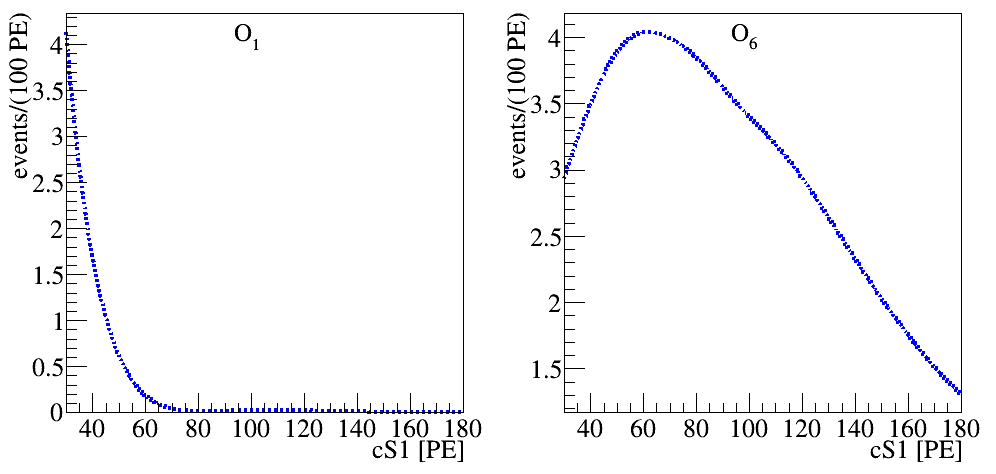
\includegraphics[width=1.\linewidth]{fig/SigHighO1O6.png}}
\end{minipage}
\mycaption[The expected signal in the high-energy region]{The expected signal in the high-energy region for a 300~GeV/$c^2$ WIMP mass, normalized to five events. Left(right) is the spectra for $O_1$($O_6$). Notice that for $O_1$ most of the events are not expected to deposit energy higher than 30~PE whereas for $O_6$ a large fraction of the events appear in this region.}
\label{fig:HighE}
\end{figure} 

\begin{figure}[h!]
\begin{minipage}{1.\linewidth}
\centerline{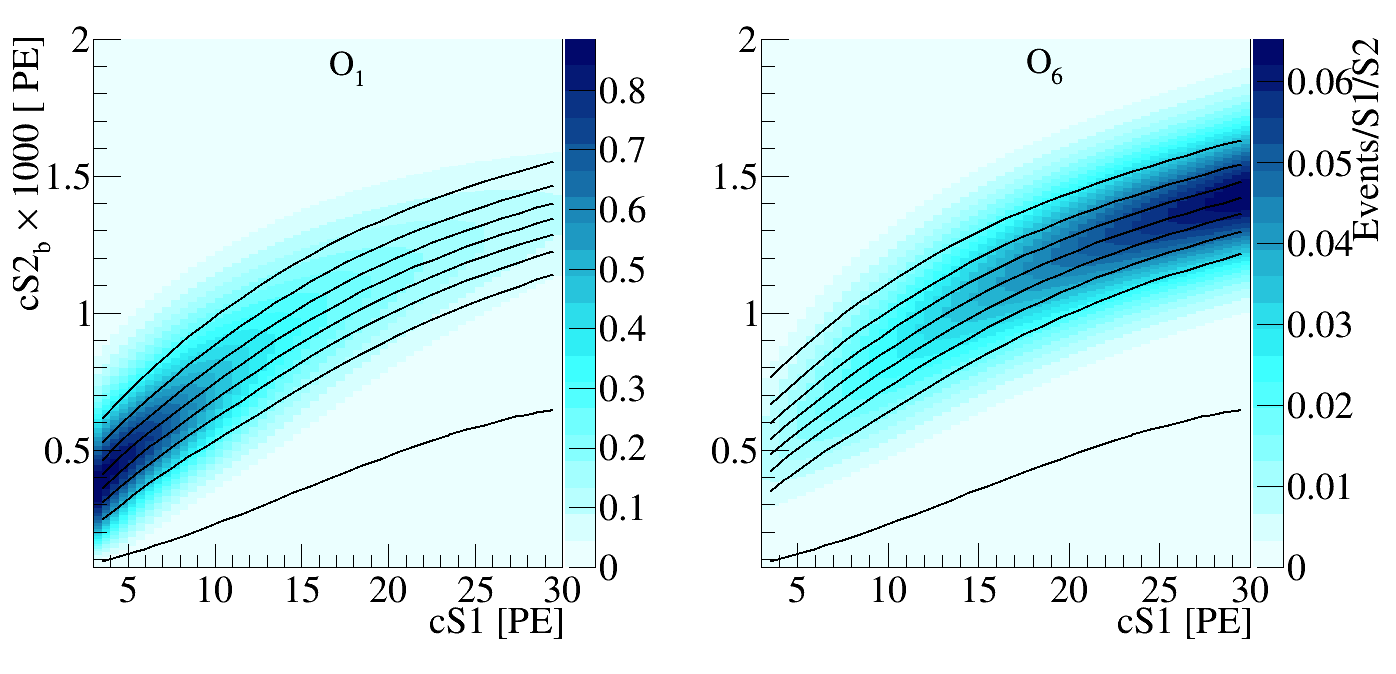
\includegraphics[width=1.\linewidth]{fig/SigLowO1O6.png}}
\end{minipage}
\mycaption[The expected signal in low energy region ]{The expected signal in the low-energy region for a 300~GeV/$c^2$ WIMP mass, normalized to five events. (a)is the spectra for $\mathcal{O}_1$ (b) is the spectra for $\mathcal{O}_6$. Notice that for $\mathcal{O}_1$ most of the events are expected to deposit energy lower than 30~PE whereas for $\mathcal{O}_6$ a large fraction of the events do not appear in this region at all. The black lines indicate the bands constructed on these specific mass and operator models, and are dividing the signal into eight equally distributed signal subregions. This parameter space can be mapped with a one-to-one mapping to the log$(cSiib/\cSi)-\cSi)$ space.
\label{fig:LowE}}
\end{figure}




\subsection{Elastic Scattering}
\label{subsubsec:Elastic}

The expected recoil energy spectrum of each WIMP mass for each EFT operator is calculated using the Mathematica package \texttt{DMFormFactor} supplied by Anand et al.~\cite{Fitzpatrick:MathTools,Anand:MathTools}. I use standard assumptions as in previous analyses (e.g \cite{xe100_run_combination}) regarding the local dark matter density and velocity distribution, namely $\rho_\mathrm{local} = 0.3$~GeV$\cdot c^{-2}$/$\mathrm{cm}^{3}$ and a Maxwell-Boltzman distribution with a mean given by the local circular velocity $v_0 = 220$ km/s and cut off at an escape velocity of $v_\mathrm{esc} = 544$ km/s. The responses of xenon nuclei to a scattering event are computed from one-body density matrices provided with the package, in contrast to the Helm form factors which have been used in previous analyses. These spectra are produced for the seven most abundant xenon isotopes (128, 129, 130, 131, 132, 134 and 136), combined in proportion to the abundance of these isotopes in the XENON detector \cite{xe100_run10_sd}, then translated into expected signal rates via the method described above.

\subsection{Inelastic WIMP Scattering}
\label{subsubsec:Inelastic}
To obtain recoil spectra for WIMP-nucleon scattering for all EFT operators with inelastic kinematics, I use a modified version of \texttt{DMFormFactor} provided by Barello et al. \cite{InelasticMath}. The authors have modified the original package to enforce the new energy conservation condition $\delta_m + \vec{v}\cdot\vec{q} + \left|\vec{q}\right|^2/2\mu_N = 0$, primarily by replacing 
$\vec{v}^\perp_{elastic} \rightarrow \vec{v}^\perp_{inelastic} = \vec{v}^\perp_{elastic} +\frac{\delta_m}{\vert{\vec{q}}\vert^2}\vec{q}$ in the definitions of the EFT and nuclear operators. 

Assumptions regarding the dark matter halo and nuclear physics are unchanged. The mass splitting $\delta_m$ between dark matter states is varied from ($0-300$)~keV, safely beyond the value at which the predicted rate is zero for the entire mass range I consider.

\section{Statistical Inference}
\label{sec:LikelihoodFunction}

The statistical interpretation of data is performed using a binned profile likelihood method, in which hypothesis testing relies upon a likelihood ratio test statistic, $\tilde{q}$, and its asymptotic distributions~\cite{asympt} to constrain the coupling constants $c_k$ for each operator $\mathcal{O}_k$. The two analysis channels are combined by multiplying their likelihoods together to produce a joint likelihood function

\begin{equation}
\label{eq:FullLikelihood}
\Llike = \Llike_{\mathrm{lowE}(c_i^2,\Qy,\Leff)} \times \Llike_{\mathrm{highE}(c_i^2,\Leff)}.
\end{equation}


Both analyses parametrize the NR relative scintillation efficiency, $\Leff$, based on existing measurements~\cite{run8Result}. Its uncertainty is the major contributor to energy scale uncertainties and is considered as correlated between the two analysis channels via a joint nuisance likelihood term.
Throughout this study, all the parameters related to systematic uncertainties are assumed to be normally distributed.

For the low-energy channel an extended likelihood function which is very similar to the one reported in~\cite{Aprile:2011hx} and described in detail in~\cite{xe100_run_combination} is employed. 
The log$(\cSiib/\cSi),\cSi{})$-plane is divided into eight WIMP mass-dependent bands where events are counted. This binned approach is extended with the corresponding \cSi{}-projected PDF of each band. The total normalization of the background is fit to data, and an uncertainty is assigned to the relative normalization of each band according to the corresponding statistical uncertainty of the calibration sample.

Signal shape variations due to energy scale uncertainty are modeled via simulation. These include  the said $\Leff$ uncertainties and additionally 
the charge yield uncertainties, which are parametrized based on $\Qy$ measurement as described in~\cite{DataMCXenon}.

The low-energy likelihood function is shown in Eq.~\ref{eq:LowELikelihood},  \begin{equation}
\label{eq:LowELikelihood}
\Llike_{lowE} = \Llike_1(c_k^2,\Leff,\Qy) \Llike_2(\epsilon_b) \Llike_3(\Leff,\Qy)
\end{equation}

\begin{equation} \label{eq:LowELikelihood1}
\begin{split}
\Llike_1(c_k^2,\Leff,\Qy) = &\prod_j Poiss(n^j|\epsilon_s^jM_s(c_k^2)+\epsilon_b^jM_b) \times  \\
&\prod_{i=1}^{n^{i,j}} \frac{\epsilon_s^j M_s(c_k^2)f_s^j(cS1^i) + \epsilon_b^j M_bf_b^j(cS1^i)}{\epsilon^j_sM_s + \epsilon^j_bM_b} ,
\end{split}
\end{equation}
where $f^j_s$ and $f^j_b$ are the probability density functions of the signal and background respectively in band j. and $M_s$ and $M_b$ are the maximum likelihood estimators for the total number of signal and background events respectively.
\begin{equation}
\Llike_2 = \prod_j Poiss(n^j_b | \epsilon_b^jN_b)
\end{equation} 

The high-energy channel analysis employs a binned likelihood function. Observed and expected event yield are compared in the nine ROI log$(\cSiib/\cSi),\cSi{})$-bins described in Sec.~\ref{subsubsec:HighE}. 
Given the large statistical uncertainty of the background model the above extended likelihood approach is not repeated here.
Instead, the maximum likelihood estimation of the background expectation in each bin is constrained by the statistical uncertainty of the calibration sample, while the total 
normalization is fit to the data. Additionally, to account for potential mis-modeling of the expected background distribution, mainly due to anomalous multiple scatter events,
a systematic uncertainty of 20\% is assigned independently to each bin. In the high-energy channel, uncertainty on the signal acceptance of analysis selections are computed for each signal hypothesis using the parametrized acceptance curve shown in Fig.~\ref{fig:Acc}.
Uncertainties on the signal model log$(\cSiib/\cSi),\cSi{})$ distribution due to $^{241}$AmBe sample statistical fluctuations, as well as energy scale shape variation due to $\Leff$ uncertainties, are taken into account.


The high-energy likelihood function is defined in Eq.~\ref{eq:HighELikelihood}
\begin{equation}
\label{eq:HighELikelihood}
\Llike_{\mathrm{highE}}(c_k^2,\Leff) = \prod_{i} \big( Poiss(n^{obs}_{i}~|~n^{s}_{i} + n^{b}_{i}) \, \times Gauss(\eta^{b}_{i}) \big) ~ \times \Llike_{stat}(\epsilon^{s}_{j},\epsilon^{b}_{i}) \times \Llike^s_{unc}(\Leff, A),
\end{equation}
where the product goes over all 9 bins, $\epsilon^{b}_{i}$ is the fraction of background event in \textbf{bin} $i$ and  $\epsilon^{s}_{j}$ is the fraction of $^{241}$AmBe data in \textbf{band} $j$. This means the uncertainty on the signal is assessed per band. $n_i^s = N_{tot}^s(c_k^2,\Leff) \times \zeta_{i,j}^s(\Leff ,\epsilon^{s}_{j})$ is the number of signal events in bin i, $\zeta_{i,j}^s(\Leff, \epsilon^{s}_{j})$ is the fraction of signal events in bin i which is in band j. $n_i^b = N_{tot}^{cal} \times \tau \times \epsilon^{b}_{i}(\eta^{b}_{i})$ is the number of background events in bin i. $\tau$ is the overall normalization of background to data, and is a free parameter.  

\section{Data From Recoil Energies Up To 1000\,PE}
\label{sec:SuperHighE}
Upon completing our analysis, I examined data in the \cSi{} region above 180\,PE, up to 1000\,PE, since it will not be analyzed in any future XENON publications. I used the same data selection criteria as those applied for the high-energy channel. These selection criteria are not optimized for the new even-higher energies and may exhibit a drop in acceptance for NRs to below 50\%. Due to the lack of NR calibration data and of a rigorous background model in this energy range, a quantitative and statistically solid inference on dark matter hypotheses is impractical. Nonetheless, I provide a plot of the data here. Fig.~\ref{fig:eft_1000} shows the distribution of science data in this extended range (in black) together with NR (in red) and ER calibration data (in blue).

\begin{figure}
\centerline{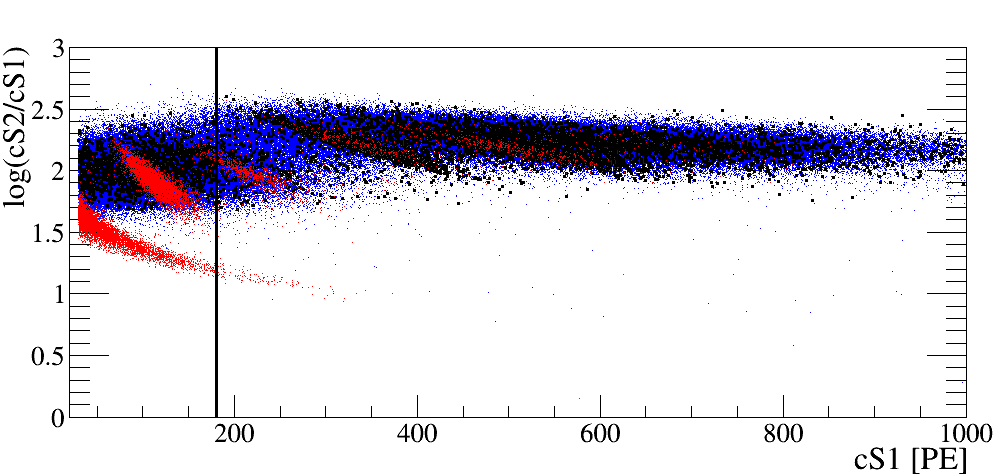
\includegraphics[width=1.\linewidth]{fig/superhighE.png}}
\mycaption[Super high energy phase space]{The full \Xehund{} dark matter science run data up to 1000~PE in \cSi{} (shown in black). In blue I show data from ER calibration ($^{60}$Co and $^{232}$Th) and in red I show data from NR calibration ($^{241}$AmBe). See the text for details on these populations. While the black vertical line represents the highest energy considered for quantitative interpretation in this analysis, there is no indication of elastic NRs even above that energy.
\label{fig:eft_1000}}
\end{figure}  

The NR calibration data show the NR band from elastic scattering, with the aforementioned loss of statistics at energies above 180\,PE clearly visible. Also visible are lines in the ER band from the inelastic scattering of neutrons on $^{129}$Xe (39.6\,keV at 130\,PE) and $^{131}$Xe (80.2\,keV at 220\,PE) as well as the delayed deexcitation of $^{131m}$Xe (169.3\,keV at 350\,PE) and $^{129m}$Xe (236.1\,keV at 500\,PE). ER calibration data are shown in blue and indicate the distribution of the prevalent background in this energy range. Since the detector is optimized for low-energy events, large S2 pulses saturate the PMT bases. This is visible in the ER band above 250\,PE.

Finally, data from the dark matter search are shown in black. As can be seen, there is no indication of elastic NRs at energies above those analyzed in this study.
 


\section{Results}
\label{sec:Results}

A benchmark region of interest is defined between the upper and lower thresholds in \cSi{} for each channel. This region
is bounded in $y$-space from above by the $^{241}$AmBe NR mean line and below by the lower 3$\sigma$ quantile of the $^{241}$AmBe neutron calibration data. The expected background in the region is $3.0 \pm 0.5_{stat}$ (low-energy) and $1.4 \pm 0.3_{stat}$ (high-energy). The number of DM candidates in this benchmark region is 3 (low-energy), and 0 (high-energy). Consequently, the data are compatible with the background-only hypothesis and no excess is found. 

For the elastic scattering case, a 90\%\,C.L.$_S$~\cite{cls} confidence level limit is set on the effective coupling constant, $c_i$,  for all operators and masses in the range of 10~GeV/$c^2$ to 1 TeV/$c^2$. The $c_i$ are dimensionful, with units of $[\mathrm{mass}]^{-2}$, so I first convert them to dimensionless quantities by multiplying them by $m_\mathrm{weak}^2=(246.2\text{ GeV})^2$, following the conventions of \cite{Anand:MathTools}. 

These limits are shown in Fig.~\ref{fig:elasticLimit} in black, along with limits from CDMS-II Si, CDMS-II Ge and SuperCDMS~\cite{CDMSEFT}.  


For the inelastic scattering case,  90\%\,C.L.$_S$ confidence level limits on the coupling constants 
(again scaled by $m_\mathrm{weak}^2$) are set. Fig.~\ref{fig:O1Inel} shows limits on the $\mathcal{O}_1$ (SI) coupling constant as a function of mass splitting and WIMP mass, Fig.~\ref{fig:InelasticLimit} shows limits for all other operators as a function of the mass splitting $\delta_m$ with a fixed WIMP mass of 1 TeV/$c^2$,  
projections of results from CDMS-II~\cite{CDMS_Inelastic}, ZEPLIN-III~\cite{Zepplin_Inel}, and \Xehund~\cite{XENON_Inelastic_WIMP} in the coupling constant and $\delta_m$ parameter space are also reported.
  

\begin{figure*}
\begin{minipage}{1.\linewidth}{}
\centerline{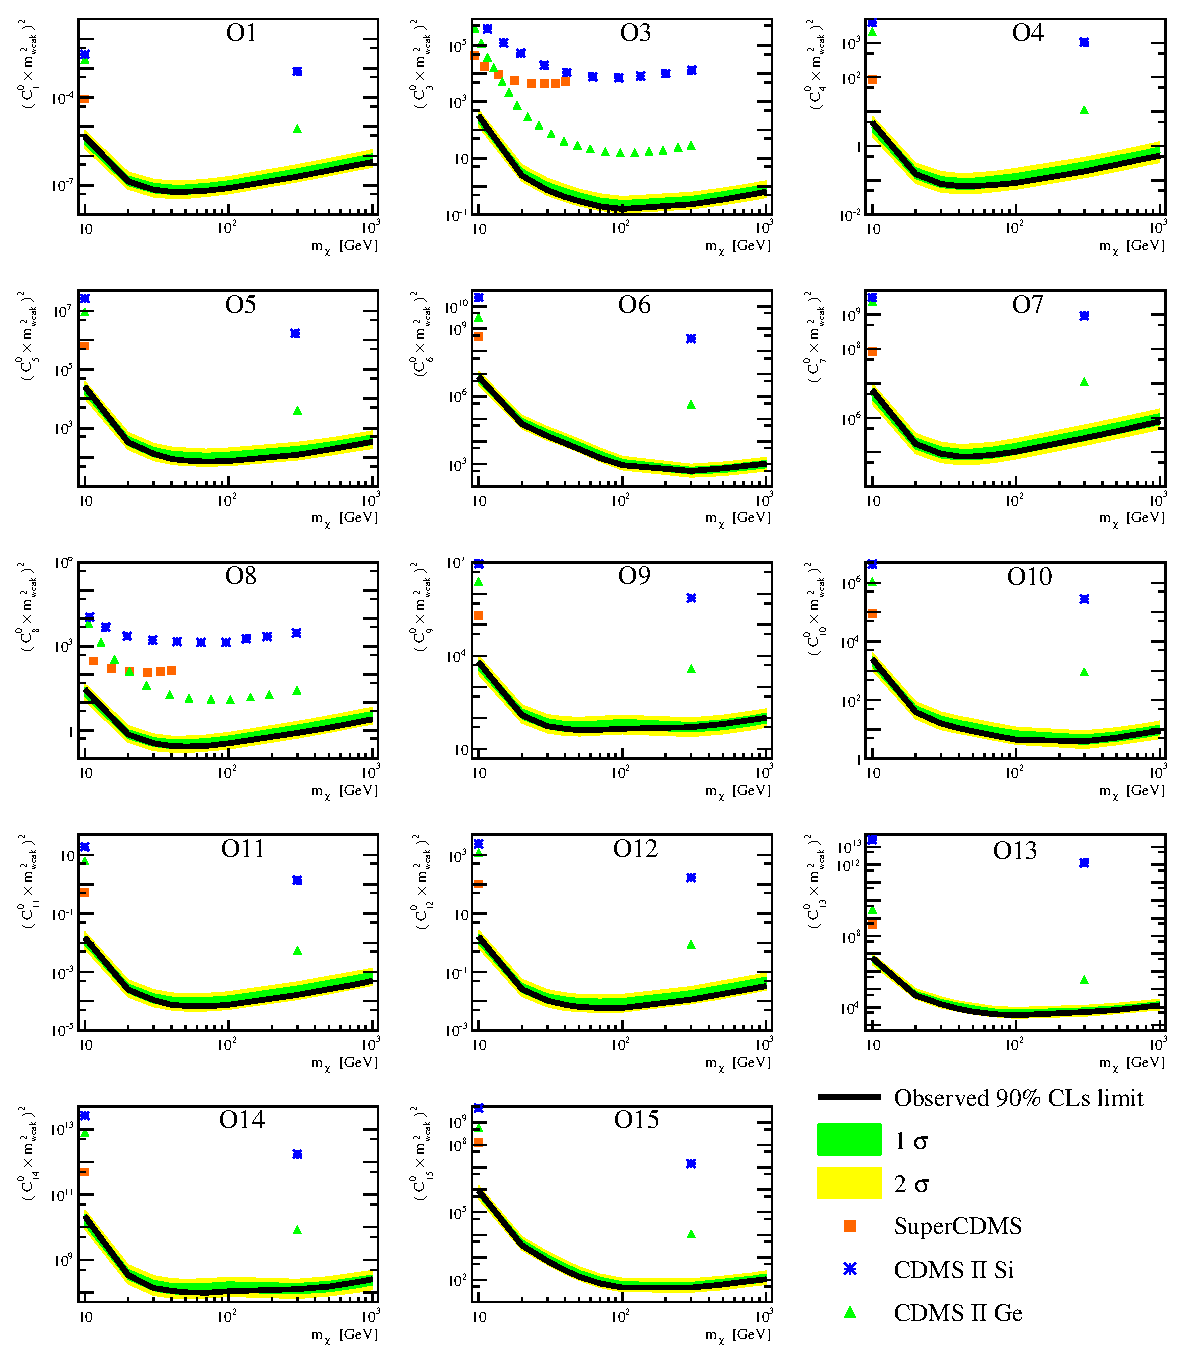
\includegraphics[width=\textwidth,height=0.99\textheight,keepaspectratio]{fig/ElasticAllLimitCDMS.pdf}}
\end{minipage}
\mycaption[The \Xehund\ limits (90\%\,C.L.$_S$) on isoscalar dimensionless coupling for all elastic scattering EFT operators]{The \Xehund\ limits (90\%\,C.L.$_S$) on isoscalar dimensionless coupling for all elastic scattering EFT operators. The limits are indicated in solid black. The expected sensitivity is shown in green and yellow(1$\sigma$ and 2$\sigma$ respectively). Limits from CDMS-II Si, CDMS-II Ge, and SuperCDMS \cite{CDMSEFT} are presented as blue asterisks, green triangles, and orange rectangles, respectively. For operators 3 and 8, a full limit was published, for all other operators only $m_\chi = 10$ and $m_\chi =300$ are available.}
\label{fig:elasticLimit}
\end{figure*}

\begin{figure}
\centerline{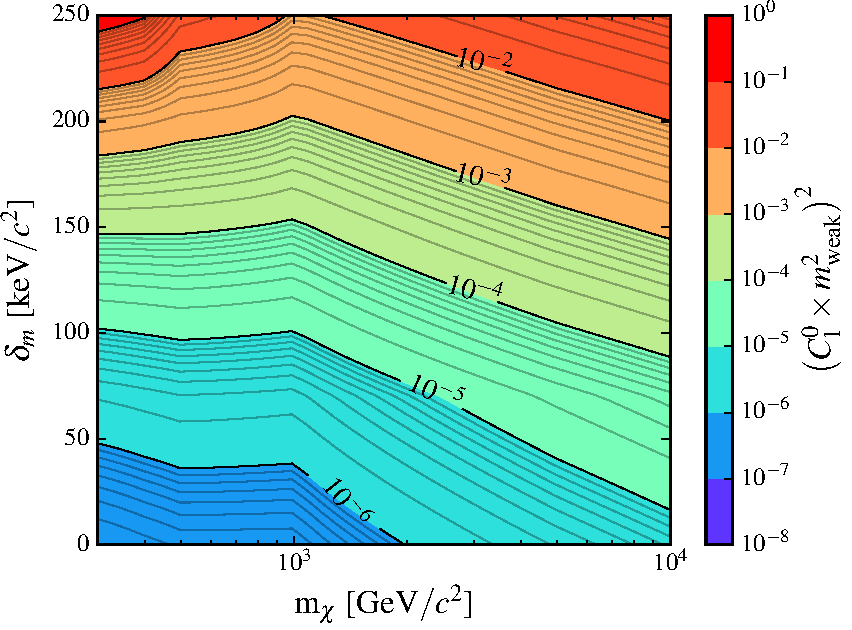
\includegraphics[width=0.7\linewidth]{fig/O1_inelastic_lim_2D.pdf}}
\mycaption[90\%\,C.L.$_S$ limits, for the inelastic model]{90\%\,C.L.$_S$ limits, for the inelastic model, on the magnitude of the coupling constant for $\mathcal{O}_1$, reported as a function of the WIMP mass and mass splitting $\delta$.}
\label{fig:O1Inel}
\end{figure}  


\begin{figure*}
\begin{minipage}{1.\linewidth}
\centerline{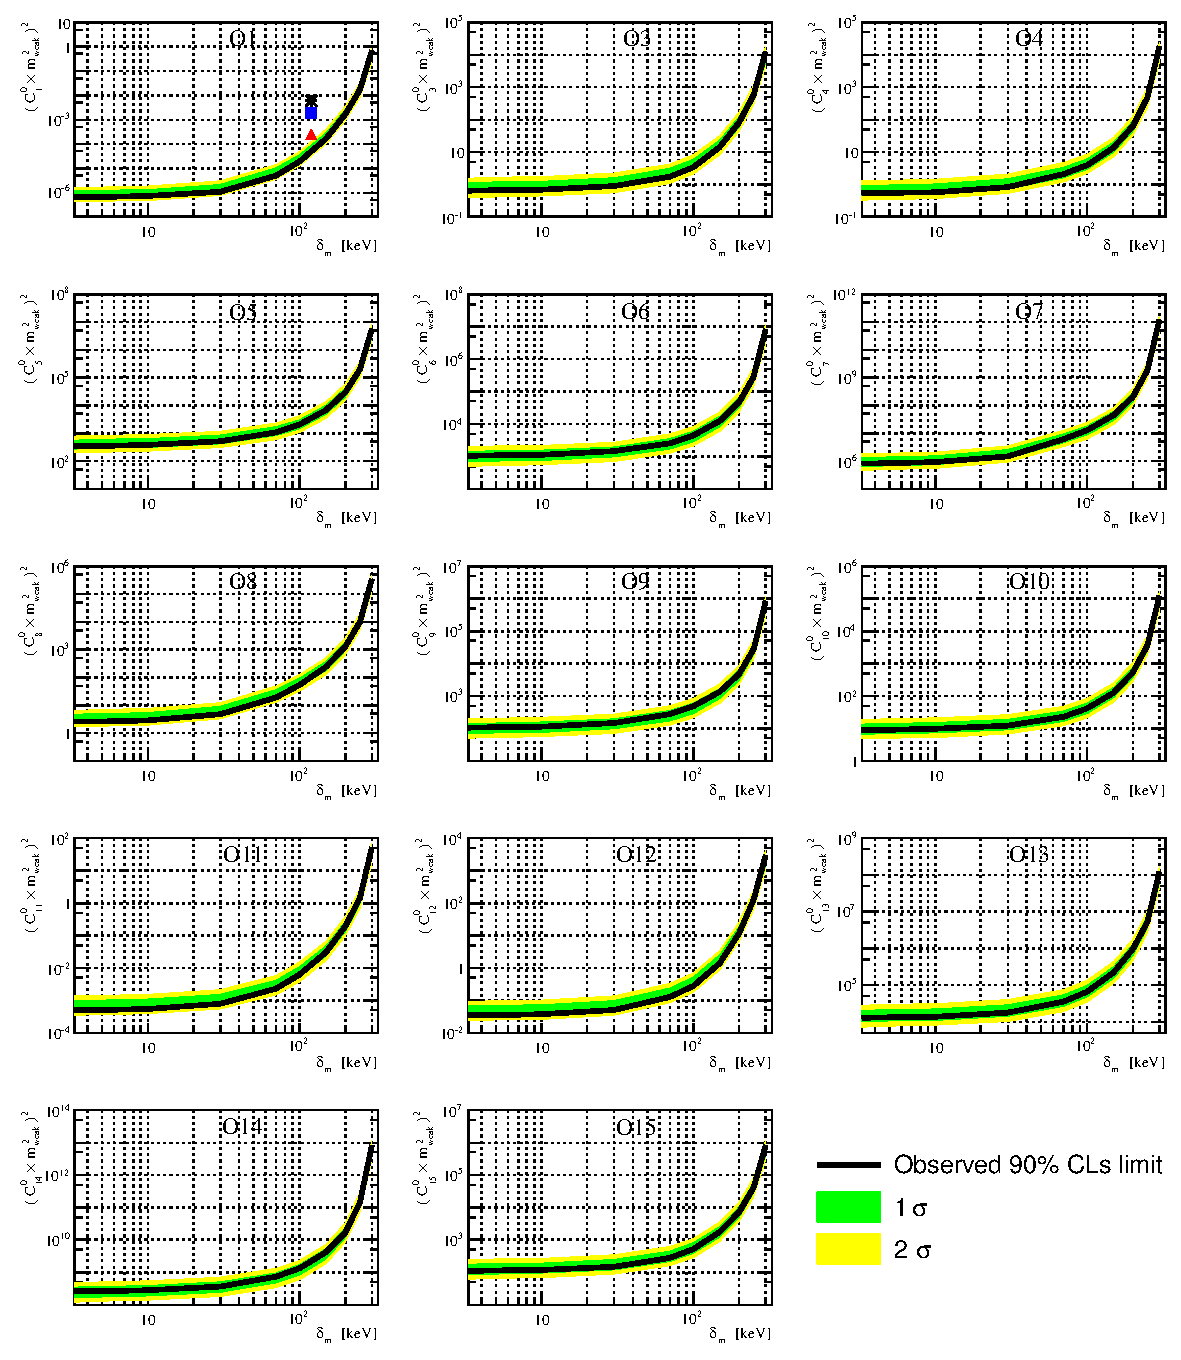
\includegraphics[width=\textwidth,height=0.99\textheight,keepaspectratio]{fig/FinalInelastic.pdf}}
\end{minipage}
\mycaption[The \Xehund\ 90\%\,C.L.$_S$ limits on a 1 TeV/$c^2$ WIMP isoscalar dimensionless coupling constant as function of the WIMP mass splitting $\delta_m$]{The \Xehund\ 90\%\,C.L.$_S$ limits on a 1 TeV/$c^2$ WIMP isoscalar dimensionless coupling constant as function of the WIMP mass splitting $\delta_m$  for all inelastic scattering EFT operators. Limits are indicated in solid black. The expected sensitivity is shown in green and yellow (1$\sigma$ and 2$\sigma$ respectively). For $\mathcal{O}_1$ (SI) results from \Xehund(red triangle) CDMS-II(blue rectangle) and ZEPLIN-III(black star) are overlaid.}
\label{fig:InelasticLimit}
\end{figure*}

For the elastic operator $O_1$, our results can be compared to those of standard SI analyses by computing the relevant zero-momentum WIMP-nucleon cross sections. This is not simple to do rigorously because the treatment of nuclear structure used in our analysis is different than in standard analyses; however, this difference is small for scattering via $O_1$. I can therefore quite safely use the ``traditional'' correspondence~\cite{DeSimone:2016fbz}
%
\begin{equation}
\sigma_{N}^\mathrm{SI} = \left(C^N_1\right)^2 \frac{\mu_{\chi,N}^2}{\pi},
\end{equation}
%
where $\mu_{\chi,N}$ is the WIMP-nucleon reduced mass. Standard SI analyses assume isospin-conserving interactions, as I do in this analysis, so I can simply set $C^N_1 = C^0_1$, such that $\sigma_{p}^\mathrm{SI}=\sigma_{n}^\mathrm{SI}$. 

In principle a similar comparison can be done between our limit on the $O_4$ coupling and standard SD analysis limits; however, this time the standard analyses do {\em not} assume isospin-conserving interactions. Instead they typically assume maximal isospin violation, that is, assuming that WIMPs couple either protons or neutrons. Limits are then derived independently on $\sigma_{p}^\mathrm{SD}$ and $\sigma_{n}^\mathrm{SD}$. Because of this difference in assumptions, our limits on SD couplings are not directly comparable to usual analyses. However, they can be recast under the appropriate alternate model assumptions using the detector response tables I provide in the supplementary material.

\section{Summary}
In this section I have presented an analysis of \textsc{Xenon100} data at
recoil energies above 43 keVnr, with the new high energy
bound set to 240 keVnr. I considered in this analysis two
models which predict interactions in this energy region:
an EFT approach for elastic WIMP-nucleon scattering,
and a similar EFT approach but considering instead inelastic WIMP-nucleon scattering. The observed data were
compatible with background expectations, and 90\% C.L.$_S$
exclusion limits were constructed for WIMP masses between (10 and 1000)\,GeV.
%
%%A figures matrix.
%\begin{figure}[t!]
%\centering
%\begin{minipage}{3.3cm}
%    \centering
%    \subtop[]{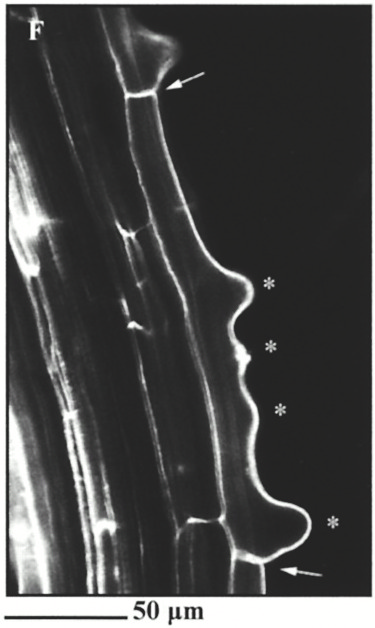
\includegraphics[height=0.28\textheight]{fig01/Nswellings}\label{sf:multiRH02a}}
%\end{minipage}
%\hspace{0.5cm}
%\begin{minipage}{3.3cm}
%    \centering
%    \subtop[]{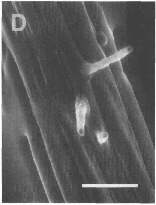
\includegraphics[height=0.27\textheight]{fig01/Mswellings}\label{sf:multiRH02b}}
%\end{minipage}
%\hspace{1.3cm}
%\begin{minipage}{3.3cm}
%    \centering
%    \subtop[]{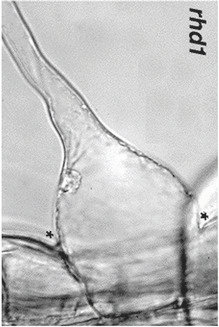
\includegraphics[height=0.27\textheight]{fig01/rhd1}\label{sf:multiRH02c}}
%\end{minipage}
%\\ \vspace{0.1cm}
%\begin{minipage}{10cm}
%    \centering
%    \subtop[]{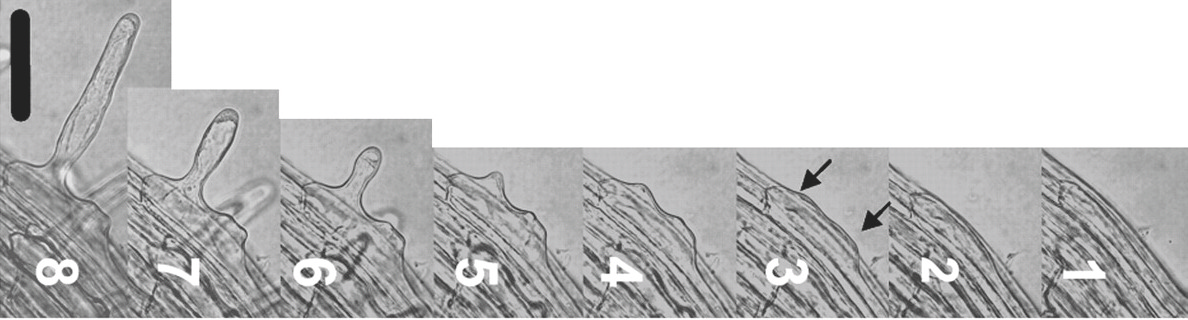
\includegraphics[height=0.145\textheight]{fig01/mutantrhd6}\label{sf:multiRH02d}}
%\end{minipage}
%\\ \vspace{0.1cm}
%\begin{minipage}{10cm}
%    \centering
%    \subtop[]{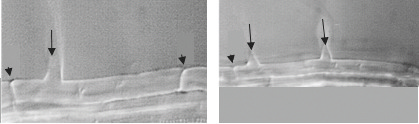
\includegraphics[height=0.16\textheight]{fig01/auxab}\label{sf:multiRH02e}}
%\end{minipage}
%\mycaption[Hair-forming mutant cells.]{(a) A mutant RH cell. Asterisks show multiple sites of RH initiation in a single root hair cell (indicated by the arrows). Figure reproduced from \cite{rigas01}. (b)~Hair-forming cell with three RH initiation locations. The bar represents $50\mu m$. Figure reproduced from \cite{massuci01}. (c) Large bump in mutant {\itshape rhd1}. Figure reproduced from \cite{griersonRH}. (d) Mutant overexpressing gene {\itshape ROP2}; from right-hand to left-hand, numbers indicate progressive snapshots at different times. RH initiation sites are indicated by the arrows. The bar represents $75\mu m$. Figure reproduced from~\cite{mjones01}. (e)~Mutants affected by auxin. On the left-hand side, RH site is farther away from the apical end (left arrow cap); on the right-hand side, multiple RH locations (arrows). Figure reproduced from~\cite{payne01}.}
%\label{fig:multiRH02}
%\end{figure}
%
%% A single figure
%\begin{figure}[t!]
%	\centering
%	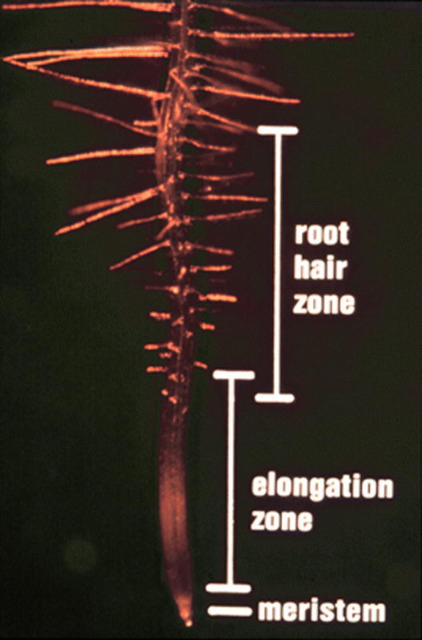
\includegraphics[height=0.35\textheight]{fig01/devepzones}
%	\mycaption[Developmental zones of an Arabidopsis root.]{Developmental zones of an Arabidopsis root. Figure reproduced from \cite{griersonRH}.}
%	\label{fig:RHP02}
%\end{figure}

%=========================================================